\begin{tikzpicture}[line cap=round,line join=round]
  \path[use as bounding box] (0,0) rectangle (13.7,10.77);
  \path[pSurface,fill=pBlueWash] (0,5.73) rectangle (6.66,10.65);
  \path[pSurface,fill=pTealWash] (7.04,5.73) rectangle (13.70,10.65);
  \path[pSurface,fill=pGoldWash] (0,.56) rectangle (6.66,5.35);
  \path[pSurface,fill=pResearchWash] (7.04,.56) rectangle (13.70,5.35);
  \pPanel{a}{Specification-based webpage}{.14}{10.33}
  \pPanel{b}{Instruction-based image editing}{7.18}{10.33}
  \pPanel{c}{Source-grounded summary}{.14}{5.02}
  \pPanel{d}{Research ablation plan}{7.18}{5.02}

  \node[pSmall,text=pInk,anchor=west] at (.22,9.84)
    {\textbf{Requirement:} an event page with a Register button.};
  \pCandidate{A}{pBlue}{.47}{9.41}
  \pCandidate{B}{pRed}{3.67}{9.41}
  \node[pSmall,anchor=west] at (.80,9.41) {Action omitted};
  \node[pSmall,anchor=west] at (4.00,9.41) {Action present};
  \foreach \x in {.25,3.46}{
    \path[draw=pBlue!45,fill=white,rounded corners=3pt]
      (\x,7.92) rectangle (\x+2.94,9.15);
    \draw[pBlue!25] (\x,8.97) -- (\x+2.94,8.97);
    \foreach \dx in {.13,.25,.37}{\fill[pSky] (\x+\dx,9.055) circle (.026);}
    \node[pLabel,text=pBlue,anchor=west] at (\x+.13,8.73) {Open Lab};
    \draw[pMuted!45] (\x+.17,8.52) -- (\x+1.28,8.52);
    \path[fill=pSky!28,rounded corners=2pt]
      (\x+1.78,8.15) rectangle (\x+2.73,8.81);
    \draw[pBlue!45] (\x+1.96,8.31) -- (\x+2.10,8.58) -- (\x+2.28,8.43)
      -- (\x+2.48,8.64);
  }
  \draw[pRed,dashed,line width=.7pt] (1.08,8.21) ellipse (.54 and .16);
  \node[pPill,fill=pSky!55,draw=pBlue!35,text=pBlue,
    minimum width=1.18cm,minimum height=.30cm] at (4.29,8.23) {Register};
  \foreach \xa/\xb in {.16/6.50,7.20/13.54}{
    \path[fill=white,rounded corners=4pt] (\xa,5.92) rectangle (\xb,7.60);
  }
  \node[pSmall,text=pInk,anchor=west] at (.30,7.33) {$H_0$: B overall};
  \node[pSmall,text=pInk,anchor=west] at (.30,6.94)
    {$\boldsymbol{H_1}$: B on requirement satisfaction};
  \node[pSmall,text=pInk,anchor=west] at (.30,6.55)
    {$H_2$: major omission in A; location: hero action};
  \node[pSmall,text=pInk,anchor=west] at (.30,6.16)
    {$H_3$: no registration path is provided};

  \node[pSmall,text=pInk,anchor=west] at (7.27,9.84)
    {\textbf{Instruction:} add a red mug; preserve the blue bowl.};
  \node[pLabel,text=pTeal] at (8.19,9.51) {Source};
  \pCandidate{A}{pBlue}{10.36}{9.51}
  \pCandidate{B}{pRed}{12.53}{9.51}
  \begin{scope}
    \clip[rounded corners=3pt] (7.22,7.97) rectangle (9.16,9.2633);
    \node[inner sep=0pt,anchor=south west] at (7.22,7.97)
      {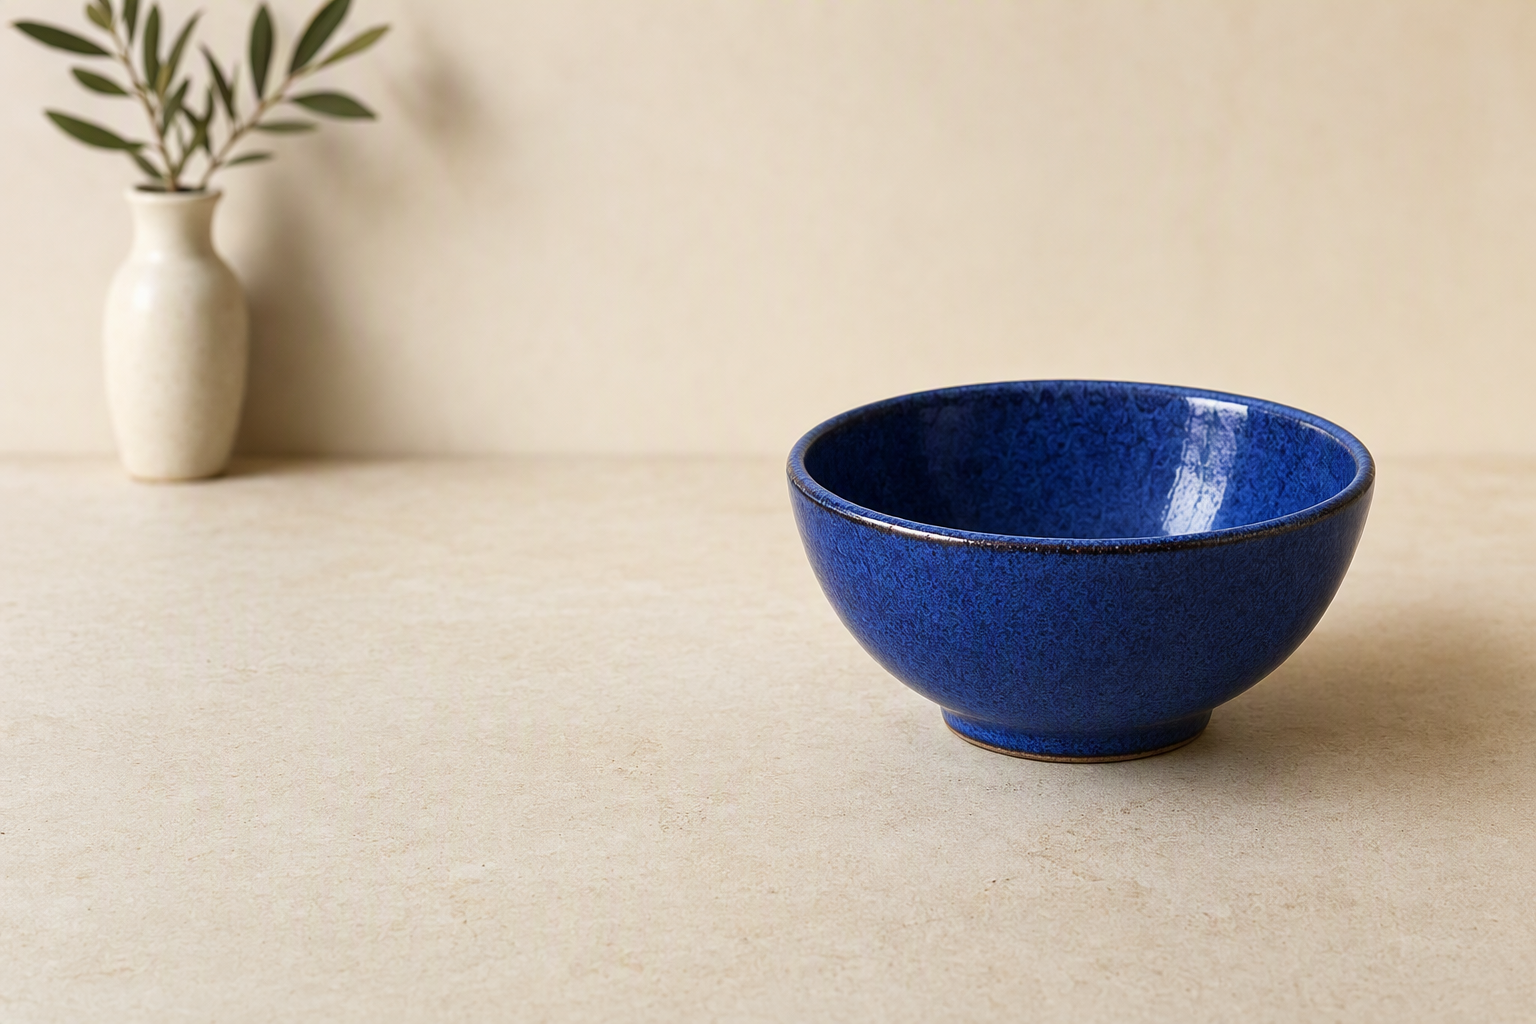
\includegraphics[width=1.94cm]{output/imagegen/edit-source.png}};
  \end{scope}
  \begin{scope}
    \clip[rounded corners=3pt] (9.39,7.97) rectangle (11.33,9.2633);
    \node[inner sep=0pt,anchor=south west] at (9.39,7.97)
      {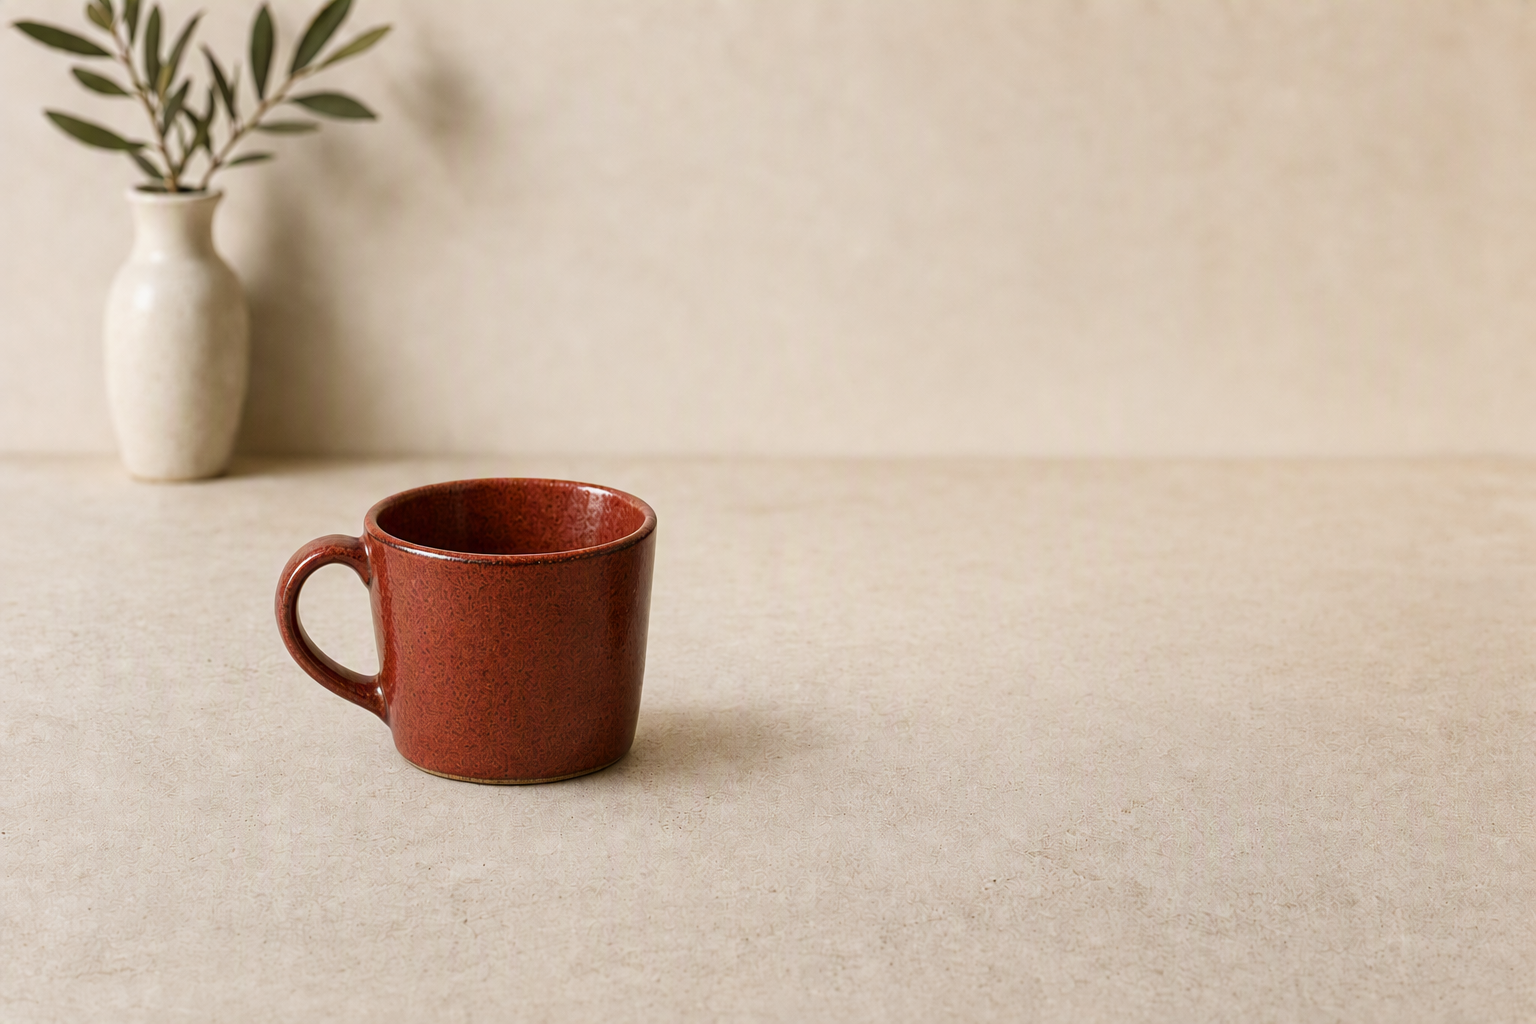
\includegraphics[width=1.94cm]{output/imagegen/edit-omission.png}};
  \end{scope}
  \begin{scope}
    \clip[rounded corners=3pt] (11.56,7.97) rectangle (13.50,9.2633);
    \node[inner sep=0pt,anchor=south west] at (11.56,7.97)
      {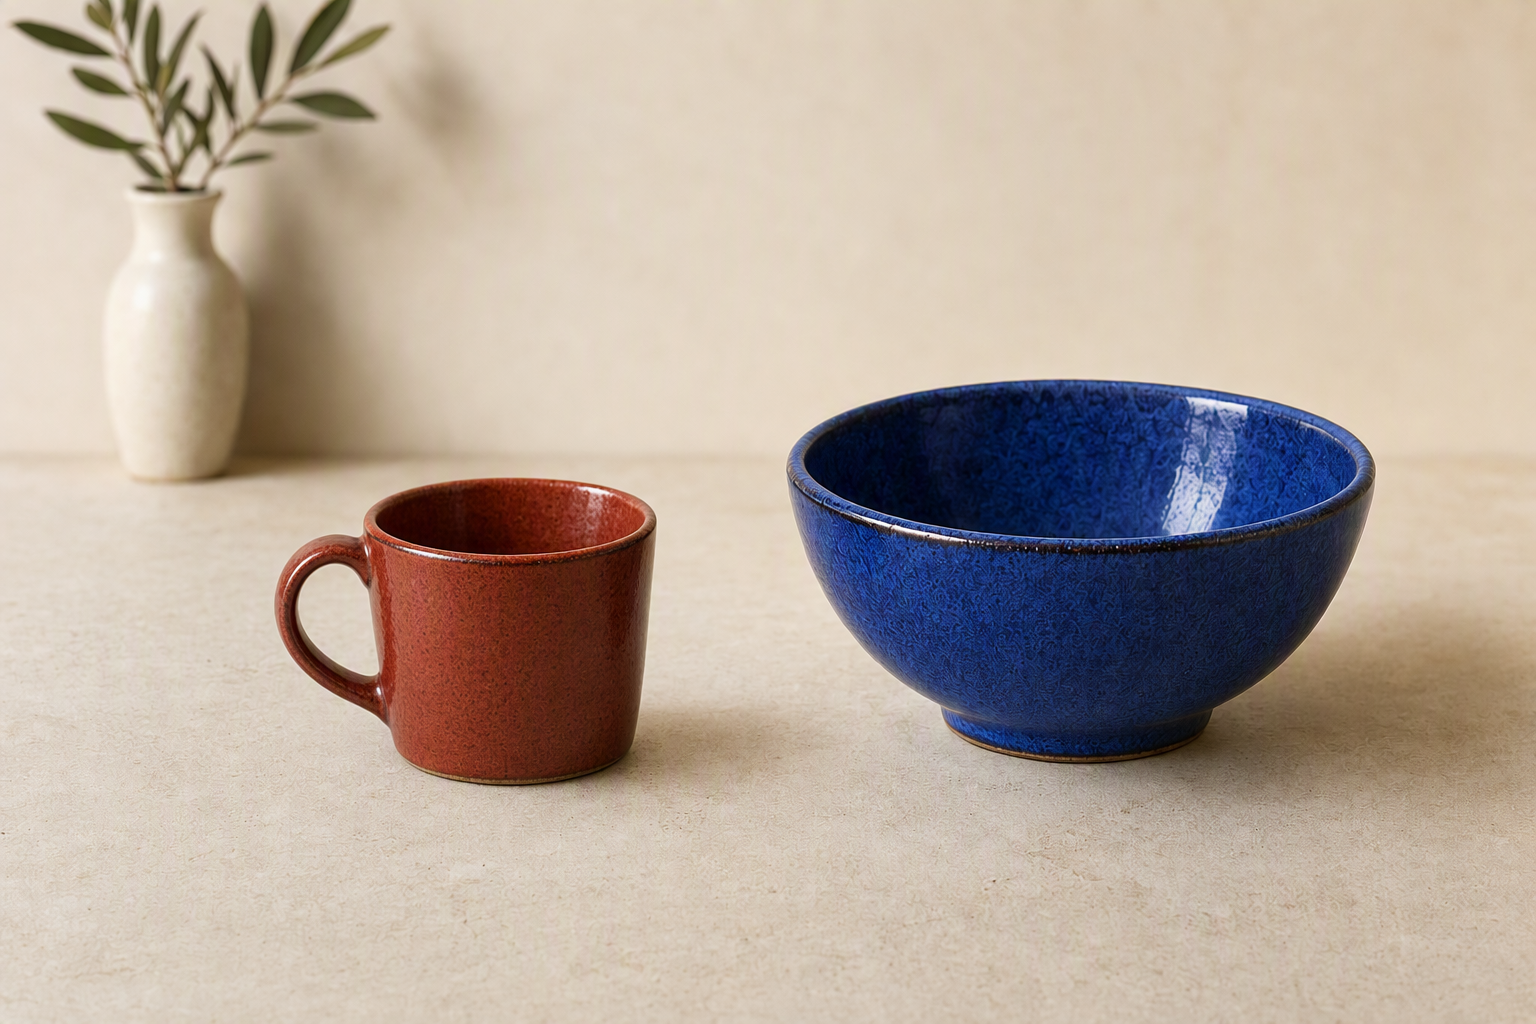
\includegraphics[width=1.94cm]{output/imagegen/edit-preserved.png}};
  \end{scope}
  \draw[pRed,densely dashed,line width=.75pt] (10.78,8.57) ellipse (.38 and .23);
  \draw[pArrow,draw=pRed] (10.78,8.34) -- (10.78,7.83);
  \node[pSmall,text=pInk,anchor=west] at (7.34,7.33) {$H_0$: B overall};
  \node[pSmall,text=pInk,anchor=west] at (7.34,6.94)
    {$\boldsymbol{H_1}$: B on preservation; tie on the added mug};
  \node[pSmall,text=pInk,anchor=west] at (7.34,6.55)
    {$H_2$: major omission in A; location: blue bowl};
  \node[pSmall,text=pInk,anchor=west] at (7.34,6.16)
    {$H_3$: an unrequested object was removed};

  \path[fill=white,rounded corners=4pt] (.16,4.15) rectangle (6.50,4.65);
  \node[pSmall,text=pInk,anchor=west] at (.30,4.40)
    {\textbf{Source:} fewer adult admissions; children not studied.};
  \pCandidate{A}{pBlue}{.40}{3.70}
  \node[pText,anchor=west] at (.76,3.70)
    {Admissions fell for \textcolor{pRed}{\underline{all age groups.}}};
  \pCandidate{B}{pRed}{.40}{3.05}
  \node[pText,anchor=west] at (.76,3.05) {Admissions fell among adults.};
  \foreach \xa/\xb in {.16/6.50,7.20/13.54}{
    \path[fill=white,rounded corners=4pt] (\xa,.75) rectangle (\xb,2.43);
  }
  \node[pSmall,text=pInk,anchor=west] at (.30,2.16) {$H_0$: B overall};
  \node[pSmall,text=pInk,anchor=west] at (.30,1.77)
    {$\boldsymbol{H_1}$: B on faithfulness};
  \node[pSmall,text=pInk,anchor=west] at (.30,1.38)
    {$H_2$: major scope error in A; location: \emph{all age groups}};
  \node[pSmall,text=pInk,anchor=west] at (.30,.99)
    {$H_3$: children were not studied};

  \node[pSmall,text=pInk,anchor=west] at (7.27,4.43)
    {\textbf{Question:} does retrieval improve factual answers?};
  \node[pSmall,anchor=west] at (7.27,4.06) {Same inputs; entries show model / retrieval};
  \pCandidate{A}{pBlue}{7.43}{3.53}
  \pCandidate{B}{pRed}{7.43}{2.95}
  \foreach \y/\left/\right/\col in {3.53/{Large / on}/{Small / off}/pRed,
    2.95/{Same / on}/{Same / off}/pTeal}{
    \node[pPill,draw=\col!40,text=\col,minimum width=2.03cm,
      minimum height=.43cm] at (9.16,\y) {\left};
    \node[pPill,draw=\col!40,text=\col,minimum width=2.03cm,
      minimum height=.43cm] at (12.13,\y) {\right};
    \node[pSmall] at (10.64,\y) {vs.};
  }
  \node[pSmall,text=pInk,anchor=west] at (7.34,2.16) {$H_0$: B overall};
  \node[pSmall,text=pInk,anchor=west] at (7.34,1.77)
    {$\boldsymbol{H_1}$: B on identifiability};
  \node[pSmall,text=pInk,anchor=west] at (7.34,1.38)
    {$H_2$: major confound in A; location: model size};
  \node[pSmall,text=pInk,anchor=west] at (7.34,.99)
    {$H_3$: retrieval is not isolated};
  \node[pSmall,align=center] at (6.85,.20)
    {Constructed tasks, candidates and judgments \quad $\vert$ \quad $H_3$ is optional human rationale, not model reasoning};
\end{tikzpicture}
